\documentclass[a5paper]{article}
\usepackage[a5paper, top=8mm, bottom=8mm, left=8mm, right=8mm]{geometry}

\usepackage{polyglossia}
\setdefaultlanguage[babelshorthands=true]{russian}

\usepackage{fontspec}
\setmainfont{FreeSerif}
\newfontfamily{\russianfonttt}[Scale=0.7]{DejaVuSansMono}

\usepackage{graphicx}
\usepackage{csquotes}

\usepackage[font=scriptsize]{caption}

\PassOptionsToPackage{hyphens}{url}\usepackage[xetex,linktocpage=true,plainpages=false,pdfpagelabels=false]{hyperref}
\hypersetup{colorlinks=true, linkcolor=blue, citecolor=blue, filecolor=blue, urlcolor=blue, pdftitle=1, pdfauthor=, pdfsubject=, pdfkeywords=}

\usepackage{tabu}

\tabulinesep=1.2mm

\sloppy

\pagestyle{plain}

\title{Возможные пути сотрудничества с кафедрой системного программирования СПбГУ}
\date{}

\begin{document}

\maketitle

\emph{Проблема} --- кадровый голод. Обилие \enquote{джунов} с низкой подготовкой после двухмесячных курсов и недостаток квалифицированных программистов.

\emph{Решение} --- подготовка специалистов под свои нужды с помощью опытных преподавателей и старейшего в стране университета.

Как именно можно участвовать:

\begin{center}
    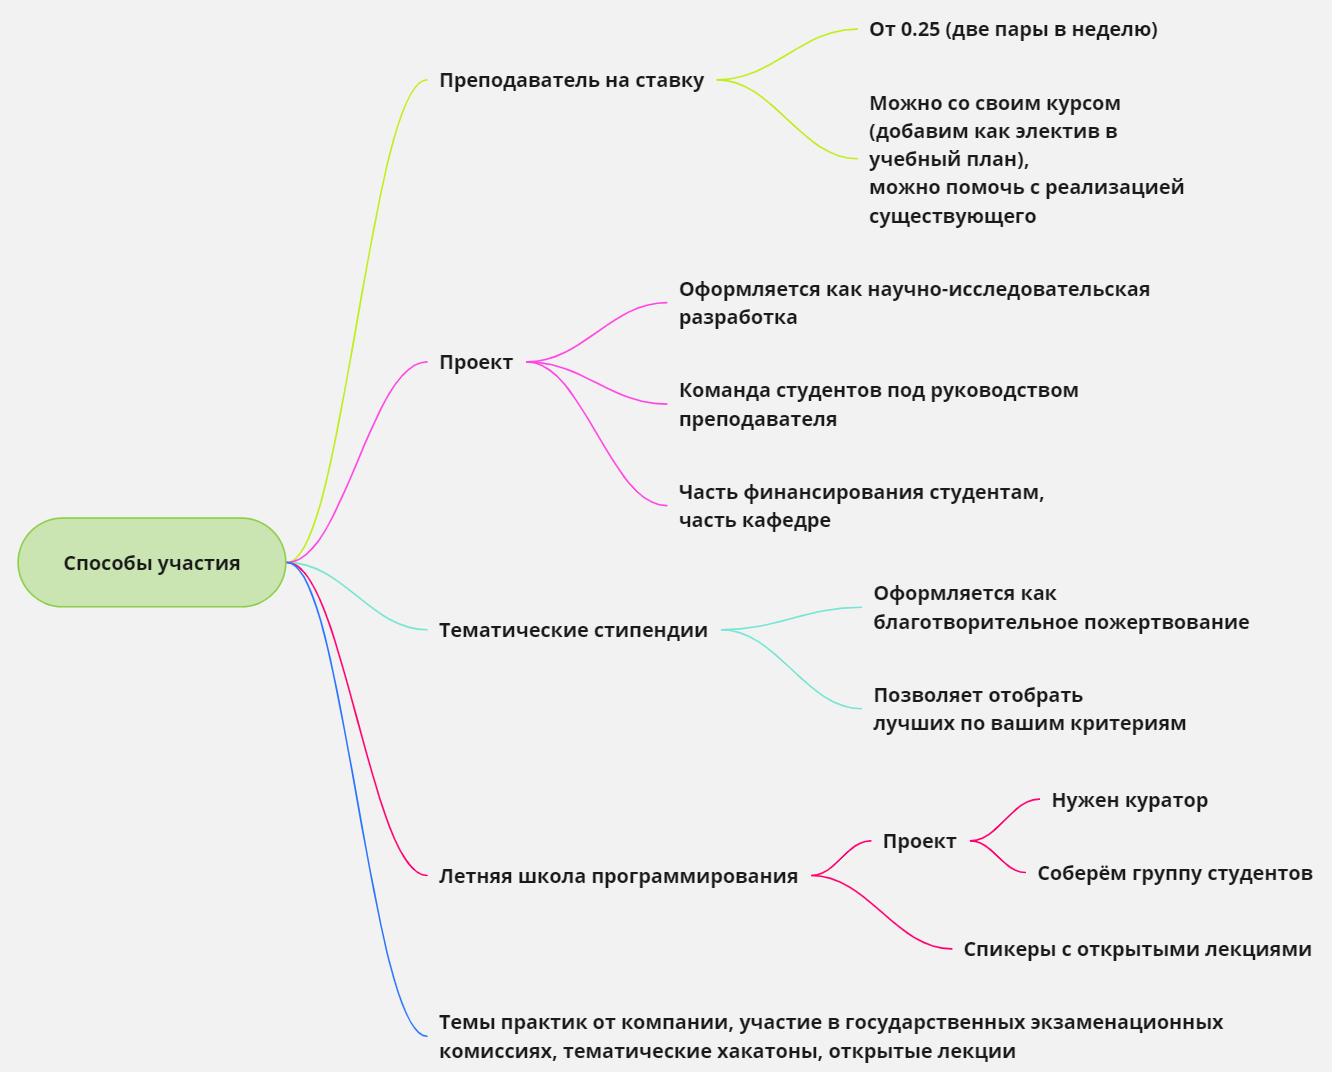
\includegraphics[width=\textwidth]{partnershipTypes.png}
\end{center}

\emph{Успешные кейсы:}

\begin{itemize}
    \item Преподавателя из штата компании имеют YADRO, ВКонтакте, Сбер, ЛАНИТ-Терком. Читают курсы, интересные компаниям, на технологиях, интересных компаниям.
    \item Стипендия YADRO, распределялась в 2023 году 20 лучшим (с точки зрения компании) студентам.
    \item Через летнюю школу программирования в 2023 году прошли более 50 студентов в 24 проектах, предложенных компаниями YADRO, Сколтехом.
    \item В государственных экзаменационных комиссиях СП директора и ведущие специалисты Яндекс, YADRO, ДоксВижн, Цифровое Проектирование, ЛАНИТ-Терком.
\end{itemize}

В одной только компании YADRO в результате сотрудничества с СПбГУ трудоустроены и успешно работают более десятка выпускников с уникальными навыками.

\emph{Почему это выгодно} --- потому что затраты вполне сравнимы с выплатой hiring bonus, но на выходе вы получаете не человека с улицы, а молодого специалиста, прошедшего несколько этапов отбора (напомним, в СПбГУ берут только лучших) и уже погружённого в вашу предметную область и технологический стек. \emph{В чём подвох} --- это небыстро. Но, говорят, не все вакансии даже людьми с улицы можно закрыть даже за год...

\section*{Подробнее}

\begin{itemize}
    \item Преподаватель на ставку --- подойдёт любой человек с высшим образованием, опыт преподавания желателен, но не обязателен. Оформление будет, скорее всего, сначала по договору гражданско-правового характера, который обеспечивает абсолютную гибкость в плане педнагрузки, но предполагает увольнение по окончанию семестра. Оформление в штат требует несколько больших формальных усилий и минимум нагрузки в две пары в неделю, но мы всегда рады новым коллегам и поможем всеми силами. Если есть готовые материалы курса --- мы готовы их интегрировать в учебный план, либо как курс по выбору с 3-го курса, либо как трек курса по программированию на 1-2 курсах. Будем рады даже прочтению пары-тройки лекций в рамках существующего курса, вполне обсуждаемо.
    \item Проект --- когда ваша компания предлагает интересную ей тему (но не критичную для продакшена) и выделяет консультанта, который будет помогать студентам. С нашей стороны обеспечивается научный руководитель, курирующий проект со стороны кафедры, мы собираем студентов, оформляем их на ставку по гранту, они работают, защищают практики, публикуются, выдают результат. Результат, скорее, весьма условный, но на выходе получается сработавшаяся команда, имеющая опыт в том, что вам нужно. Как стажировка, только у нас и с минимальным отвлечением ваших ресурсов. Чтобы это хорошо работало, нужно некоторое финансирование, которое мы умеем проводить через СПбГУ как заказную НИОКР.
    \begin{itemize}
        \item Также возможен и обратный вариант --- когда кто-то из ваших подопечных студентов или стажёров присоединяется к какому-то из интересных вам наших существующих проектов, чтобы получить опыт практической и научной работы, и сделать нам что-то полезное. Например, у нас есть сложившиеся коллективы, хорошо умеющие писать на современном C++ или работать с платами.
    \end{itemize}
    \item Стипендии --- когда мы вместе разрабатываем набор критериев выплаты стипендии, проводим открытый конкурс, распределяем стипендии среди студентов, повышаем их лояльность вам как работодателю и творим добро. Это не так дорого, как кажется --- стипендия может быть единовременной выплатой, студентам будет приятна любая сумма, параметры стипендии определяете вы. Деньги на выплаты мы умеем проводить через СПбГУ как договор пожертвования.
    \item Летняя школа --- это ежегодное мероприятие, которое проводится в июле и предполагает проектную работу студентов плюс \emph{научно-развлекательную} лекционную программу. Чтобы в ней поучаствовать, можно предложить идею проекта примерно на 20 часов в неделю на месяц для команды от одного до где-то пяти неопытных разработчиков, выделить человека, который будет читать их код и наставлять на путь истинный, и связаться с нами, чтобы мы добавили проект в программу. Можно договориться о призах и подарках участникам. Также будем рады открытой лекции в рамках летней школы (на час-полтора) по какой-нибудь интересной и нам, и вам теме.
    \item Темы практик --- у нас есть целый отдельный документ с описанием процесса практик, \url{https://disk.yandex.ru/i/PfaFf4QN-3aWvA}. Если кратко, то это что-то вроде НИОКР, но бесплатно и менее масштабно, плюс в жёстких временных рамках. От вас потребуется интересная тема, которую вы должны быть готовы представить в сентябре (или в феврале, но в феврале существенно меньше шансов найти исполнителя) и консультант, который будет работать со студентом. От нас --- курирование работы со стороны кафедры. На выходе получаете хорошего кандидата на стажировку, с которым уже минимум полгода поработали (а то и не одного).
    \item Участие в ГЭК или комиссиях по практикам --- всё то, что раньше называлось \enquote{диплом} или \enquote{курсовая} сейчас обязательно защищается перед комиссией из представителей работодателей, в конце каждого семестра. Наиболее престижно участвовать в ГЭК, однако в комиссиях по практикам можно раньше начать общаться со студентами (практики у нас со второго курса), присмотреться к интересным кандидатам, позвать делать следующую работу к себе. На эту форму сотрудничества вы тратите где-то один день в год, но получаете возможность посмотреть, чем на нашей кафедре занимаются, какого уровня у нас работы, и пообщаться со студентами в рамках защиты. Это хорошая опция для начала сотрудничества.
    \item Тематические хакатоны --- можно попробовать организовать с нашей помощью хакатон на один-три дня с призами победителям, по интересной вам (и нам) теме. От вас потребуется задача и консультант, который будет работать со студентами, мы обеспечим рекламу мероприятия, предоставим площадку.
    \item Открытая лекция или выступление на семинаре --- когда вы согласуете с нами тему лекции, приходите и рассказываете что-то интересное студентам. Правда, это не может быть неприкрытой рекламой вашей компании или рассказ о том, как попасть к вам на стажировку --- для этого у нас есть факультетская неделя карьеры, в первых числах марта. Кстати, на факультетской неделе карьеры тоже вполне можно выступить, будем рады.
\end{itemize}

Абсолютно все активности, кроме, разве что, работы преподавателем на ставке, можно вести удалённо.

\section*{Куда обращаться}

Если вы хотите:

\begin{itemize}
    \item Заключить рамочный договор о сотрудничестве с СПбГУ или договор о практиках --- пишите Амелиной Ольге Константиновне (o.amelina@spbu.ru), заместителю начальника отдела практик и содействия трудоустройству по нашему направлению. Можно ставить в копию Якова Александровича Кириленко (y.kirilenko@spbu.ru) для ускорения процесса.
    \item Предложить тему выпускной квалификационной работы или практики --- отправьте её на рассмотрение через сервис \url{https://se.math.spbu.ru/diplomas/}. Также стоит связаться с кем-нибудь с кафедры и обсудить предложенную тему и формат сотрудничества. Связаться можно с Яковом Александровичем Кириленко (y.kirilenko@spbu.ru) или Юрием Викторовичем Литвиновым (y.litvinov@spbu.ru, \url{https://t.me/yurii_litvinov}).
    \item Принять участие в государственных экзаменационных комиссиях или в комиссиях по учебным практикам --- пишите координатору ГЭК и практик Юрию Викторовичу Литвинову (y.litvinov@spbu.ru, \url{https://t.me/yurii_litvinov}).
    \item По летней школе --- тоже Юрию Викторовичу Литвинову (y.litvinov@spbu.ru, \url{https://t.me/yurii_litvinov}).
    \item Во всех остальных случаях --- Якову Александровичу Кириленко (y.kirilenko@spbu.ru).
\end{itemize}

\end{document}